\documentclass[10pt,letterpaper,english,hidelinks]{amsart}

\usepackage{amsmath}
\usepackage{amssymb}
\usepackage{amsthm}
\usepackage{fancyhdr}
\usepackage{graphicx}
\usepackage{pgfplots}
\usepackage{tikz}
\usepackage{datetime2}
\usepackage{natbib}
\usepackage[unicode]{hyperref}
\usepackage{mathtools}
\mathtoolsset{showonlyrefs}

\usetikzlibrary{fadings}
\usetikzlibrary{patterns}
\usetikzlibrary{shadows.blur}
\usetikzlibrary{arrows}
\usetikzlibrary{decorations.markings}
\usetikzlibrary{positioning}
\usetikzlibrary{calc}
\usetikzlibrary{math}

\pgfplotsset{compat=1.16}

\DTMnewdatestyle{mydateformat}{%
  \renewcommand{\DTMdisplaydate}[4]{%
    \number##1\ % year
    \DTMenglishmonthname{##2}\ % Month
    \number##3% day
  }%
  \renewcommand{\DTMDisplaydate}{\DTMdisplaydate}%
}
\DTMsetdatestyle{mydateformat}

% text dimensions
\setlength{\textwidth}{6.5in}
\setlength{\textheight}{9in}

% adjust top margins
\setlength{\topmargin}{0in}
\setlength{\voffset}{-30pt}
\setlength{\headheight}{12pt}

% no room for notes on the side
\setlength{\oddsidemargin}{0in}
\setlength{\evensidemargin}{0in}
\setlength{\marginparwidth}{0in}

% space between paragraphs and lines
\setlength{\parskip}{5pt}
\linespread{1.05} % for final submission
% \linespread{2} % for editing drafts

% Hyphenation
\numberwithin{equation}{section}
\hyphenation{semi-stable}

% Numbering for Theorems, Lemmas, etc.
\theoremstyle{plain}
\newtheorem{theorem}{Theorem}[section]
\newtheorem{corollary}[theorem]{Corollary}
\newtheorem{lemma}[theorem]{Lemma}
\newtheorem{conjecture}[theorem]{Conjecture}
\theoremstyle{definition}
\newtheorem{definition}[theorem]{Definition}
\newtheorem{example}[theorem]{Example}
\newtheorem{remark}[theorem]{Remark}
\numberwithin{equation}{section}

% Header Definitions
\fancyhead[L]{\nouppercase{\rightmark}}
\fancyhead[R]{\nouppercase{\leftmark}}

\pagestyle{fancy}

\newcommand{\cech}{\v{C}ech }
\DeclareMathOperator{\Cech}{\textrm{\v{C}ech}}
\DeclareMathOperator{\Ima}{Im}
\DeclareMathOperator{\Ker}{Ker}
\DeclareMathOperator{\nul}{Null}
\DeclareMathOperator{\boundary}{\partial}
\newcommand*{\Z}{\mathbb{Z}}
\newcommand{\bigslant}[2]{%
  \mathchoice
  {{\raisebox{.2em}{$#1$}\left/\raisebox{-.2em}{$#2$}\right.}}
  {{\raisebox{0em}{$#1$}\left/\raisebox{0em}{$#2$}\right.}}
  {{\raisebox{0em}{$#1$}\left/\raisebox{0em}{$#2$}\right.}}
  {{\raisebox{0em}{$#1$}\left/\raisebox{0em}{$#2$}\right.}}
}
\newcommand{\cross}{\times}
\newcommand{\normalsubgroup}{\triangleleft}
\newcommand{\figref}[1]{[Fig. \ref{#1}]}
\newcommand{\subfigref}[2]{[Fig. \ref{#1}, #2]}
\newcommand{\red}[1]{{\color{red} #1}}
\newcommand{\lightgray}[1]{{\color{lightgray} #1}}


\title[Persistent Homology]{Persistent Homology: Computations and Applications}
\author{Stephen Ermshar}
\address{Walla Walla University}
\thanks{Advisor: Dr. John Foster}

\date{\DTMDisplaydate{2020}{5}{15}{}} % first draft due

\begin{document}

\begin{abstract}
    % 300 word abstract.
    Persistent Homology is a method for understanding a numerical multi dimensional data set by observing certain features of shapes generated by the data.
    These features of interest are holes, and can provide clues for how the data is connected or where data may be missing.
    Homology is the study of these holes, and Persistent Homology is a natural application of this topic to data sets.
    This paper will provide an introduction to Simplicial Homology and how it can be applied to a data set.
\end{abstract}
\maketitle

\section{Introduction}

Given a collection of points in three or fewer dimensions, a person can easily make useful observations about the general shape of the data.
For instance, the points may appear to form distinct components, loops \figref{fig:annulus}, or hollow shapes.
These are examples of shapes with zero, one, and two dimensional holes, respectively.

\begin{figure}
    \tikzset{every picture/.style={line width=0.75pt}} %set default line width to 0.75pt

\begin{tikzpicture}[x=0.75pt,y=0.75pt,yscale=-0.5,xscale=0.5]
    \begin{scope}[shift={(-200,0)}]
        \begin{axis}[
            axis line style={draw=none},
            tick style={draw=none},
            yticklabels={,,},
            xticklabels={,,}
        ]
        \addplot table [scatter, only marks, x=x, y=y, col sep=comma] {tikz/annulus-point-cloud-data.csv};
        \end{axis}
    \end{scope}

    \draw[->] (100, 100) -- (150, 100);

    \begin{scope}[shift={(-120,-40)}]
        \draw  [draw opacity=0][fill={rgb, 255:red, 74; green, 144; blue, 226 }  ,fill opacity=1 ,even odd rule] (357,153.5) .. controls (357,121.19) and (383.19,95) .. (415.5,95) .. controls (447.81,95) and (474,121.19) .. (474,153.5) .. controls (474,185.81) and (447.81,212) .. (415.5,212) .. controls (383.19,212) and (357,185.81) .. (357,153.5)(329,153.5) .. controls (329,105.73) and (367.73,67) .. (415.5,67) .. controls (463.27,67) and (502,105.73) .. (502,153.5) .. controls (502,201.27) and (463.27,240) .. (415.5,240) .. controls (367.73,240) and (329,201.27) .. (329,153.5) ;
    \end{scope}
\end{tikzpicture}

    \caption{A collection of points that form a loop.}
    \label{fig:annulus}
\end{figure}

In higher dimensions such features cannot be easily observed by a person, additionally, it would be convenient to have a method for recognizing holes of any dimension.
To accomplish this goal in familiar dimensions a person might recognize that points near each other are associated with each other.
A natural first step would be to begin connecting pairs of points that are near each other with lines, this can be generalized to larger sets of points as well.
Sets of three points near each other can be connected with a triangle, sets of four with a tetrahedron, and so on. A collection of these sets forms a simplicial complex on which we can apply methods from homology to find holes.

When connecting the points in a data set different shapes may result depending on how close points must be to connect them.
If this closeness requirement is too small then no points will be connected, and if it is too large, then all points will be connected.
In either case no useful information about the structure of the data set is achieved.
Instead, the most significant structures will be detected at a wide range of scales, so persistent homology calculates homology at multiple scales to find which features persist the most.

This paper will first introduce a method for building a simplicial complex from a set of points, and \red{may explore alternate methods}.
Section \ref{sec:homology} will introduce the topic of simplicial homology, and calculate the homology group for an example simplicial complex.
Section \ref{sec:per-hom} will show how calculating homology for complexes at multiple scales produces descriptive visualizations of the data, even in high dimensions.
And Finally, Section \ref{sec:appls} will provide examples of cases where the visualizations produced by persistent homology provided meaningful information about a data set.

% Given a collection of points in \(n\)-dimensional space, we want to reveal qualitative properties of an underlying shape that the points may have been sampled from.

% \begin{figure}[h!]
%     \centering
%     \tikzset{every picture/.style={line width=0.75pt}} %set default line width to 0.75pt

\begin{tikzpicture}[x=0.75pt,y=0.75pt,yscale=-0.5,xscale=0.5]
    \begin{scope}[shift={(-200,0)}]
        \begin{axis}[
            axis line style={draw=none},
            tick style={draw=none},
            yticklabels={,,},
            xticklabels={,,}
        ]
        \addplot table [scatter, only marks, x=x, y=y, col sep=comma] {tikz/annulus-point-cloud-data.csv};
        \end{axis}
    \end{scope}

    \draw[->] (100, 100) -- (150, 100);

    \begin{scope}[shift={(-120,-40)}]
        \draw  [draw opacity=0][fill={rgb, 255:red, 74; green, 144; blue, 226 }  ,fill opacity=1 ,even odd rule] (357,153.5) .. controls (357,121.19) and (383.19,95) .. (415.5,95) .. controls (447.81,95) and (474,121.19) .. (474,153.5) .. controls (474,185.81) and (447.81,212) .. (415.5,212) .. controls (383.19,212) and (357,185.81) .. (357,153.5)(329,153.5) .. controls (329,105.73) and (367.73,67) .. (415.5,67) .. controls (463.27,67) and (502,105.73) .. (502,153.5) .. controls (502,201.27) and (463.27,240) .. (415.5,240) .. controls (367.73,240) and (329,201.27) .. (329,153.5) ;
    \end{scope}
\end{tikzpicture}

%     \caption{Motivation Example}
% \end{figure}

% High-dimensional data can be extracted from many sources, including images, health-data, and signals.

\section{Homology}\label{sec:homology}

To find a hole we first need to define what a hole is.

Homology is an abstraction that uses the concept of paths that form cycles in a space to look for paths that cannot be shrunk down to a single point.
In general, to do this we'll find all possible cycles, and factor out those that surround solid areas of the space, leaving those that surround gaps.

\begin{definition}
    The \textbf{n-th Homology Group} is \(H_n = \bigslant{\Ker(\partial_n)}{\Ima(\partial_{n+1})}\)
    \cite{fraleigha}.
\end{definition}

% \begin{definition}\label{defcechcomp}
%     Given a set of points \(P\), and a distance \(r\), let \(B_x(r)\) be the ball with radius \(r\) around the point \(x\).
%     \begin{align*}
%         \textrm{\v{C}ech}(r) := \{ S \subseteq P | \bigcap_{x\in S} B_x(r) \neq \emptyset \}
%     \end{align*}
%     \cite{wagner}
% \end{definition}

\subsection{Simplicial Homology}\label{subsec:simpl-hom}

\begin{figure}
    \tikzset{
pattern size/.store in=\mcSize,
pattern size = 5pt,
pattern thickness/.store in=\mcThickness,
pattern thickness = 0.3pt,
pattern radius/.store in=\mcRadius,
pattern radius = 1pt}
\makeatletter
\pgfutil@ifundefined{pgf@pattern@name@_iy1rqtf17}{
\pgfdeclarepatternformonly[\mcThickness,\mcSize]{_iy1rqtf17}
{\pgfqpoint{0pt}{0pt}}
{\pgfpoint{\mcSize+\mcThickness}{\mcSize+\mcThickness}}
{\pgfpoint{\mcSize}{\mcSize}}
{
\pgfsetcolor{\tikz@pattern@color}
\pgfsetlinewidth{\mcThickness}
\pgfpathmoveto{\pgfqpoint{0pt}{0pt}}
\pgfpathlineto{\pgfpoint{\mcSize+\mcThickness}{\mcSize+\mcThickness}}
\pgfusepath{stroke}
}}
\makeatother
\tikzset{every picture/.style={line width=0.75pt}}

\begin{tikzpicture}[x=0.75pt,y=0.75pt,yscale=-1,xscale=1]
    \begin{scope}[very thick,decoration={
        markings,
        mark=at position 0.5 with {\arrow{latex}}},
        decorate
    ]
    \coordinate (1) at (-60,0);
    \coordinate (3) at (0,-30);
    \coordinate (2) at (0,30);
    \coordinate (4) at (60,0);
    \coordinate (rotator) at (-27,-4);

    \draw (1)--(2) ;
    \draw (1)--(3) ;
    \draw (2)--(3) ;
    \draw (2)--(4) ;
    \draw (3)--(4) ;

    \draw (1) circle [x radius= 3.35, y radius= 3.35]
            [fill={rgb, 255:red, 0; green, 0; blue, 0 }  ]
            node[below left=3 of 1] {1}  ;
    \draw (2) circle [x radius= 3.35, y radius= 3.35]
            [fill={rgb, 255:red, 0; green, 0; blue, 0 }  ]
            node[below right=3 of 2] {2}  ;
    \draw (3) circle [x radius= 3.35, y radius= 3.35]
            [fill={rgb, 255:red, 0; green, 0; blue, 0 }  ]
            node[above right=3 of 3] {3}  ;
    \draw (4) circle [x radius= 3.35, y radius= 3.35]
            [fill={rgb, 255:red, 0; green, 0; blue, 0 }  ]
            node[below right=3 of 4] {4}  ;

    \draw [pattern=_iy1rqtf17,pattern size=6pt,pattern thickness=0.75pt,pattern radius=0pt, pattern color={rgb, 255:red, 0; green, 0; blue, 0}]
    (1) -- (2) -- (3) -- cycle ;

    \draw [stealth-] (rotator) arc (-150:150:8 and 8);

	\end{scope}
\end{tikzpicture}

    \caption{A small simplicial complex with a single one dimensional cycle.}
    \label{fig:4pt-comp-1}
\end{figure}

Homology can be efficiently calculated on simplicial complexes using familiar tools from linear and abstract algebra.

To demonstrate homology calculations we'll start with an existing simplicial complex \figref{fig:4pt-comp-1}.

\begin{figure}
    \scalebox{.8}{
        

\tikzset{every picture/.style={line width=0.75pt}} %set default line width to 0.75pt

\begin{tikzpicture}[x=0.75pt,y=0.75pt,yscale=-1,xscale=1]
%uncomment if require: \path (0,300); %set diagram left start at 0, and has height of 300

%Shape: Ellipse [id:dp027523575399996947]
\draw  [fill={rgb, 255:red, 50; green, 115; blue, 190 }  ,fill opacity=1 ] (172.13,80.75) .. controls (172.13,52.45) and (183.06,29.5) .. (196.54,29.5) .. controls (210.02,29.5) and (220.94,52.45) .. (220.94,80.75) .. controls (220.94,109.05) and (210.02,132) .. (196.54,132) .. controls (183.06,132) and (172.13,109.05) .. (172.13,80.75) -- cycle ;
%Shape: Ellipse [id:dp6715234856450412]
\draw   (1,79.75) .. controls (1,36.26) and (17.79,1) .. (38.5,1) .. controls (59.21,1) and (76,36.26) .. (76,79.75) .. controls (76,123.24) and (59.21,158.5) .. (38.5,158.5) .. controls (17.79,158.5) and (1,123.24) .. (1,79.75) -- cycle ;
%Shape: Ellipse [id:dp5970693035579542]
\draw   (159,80.75) .. controls (159,37.26) and (175.79,2) .. (196.5,2) .. controls (217.21,2) and (234,37.26) .. (234,80.75) .. controls (234,124.24) and (217.21,159.5) .. (196.5,159.5) .. controls (175.79,159.5) and (159,124.24) .. (159,80.75) -- cycle ;
%Shape: Ellipse [id:dp677120237183229]
\draw   (311,79.75) .. controls (311,36.26) and (327.79,1) .. (348.5,1) .. controls (369.21,1) and (386,36.26) .. (386,79.75) .. controls (386,123.24) and (369.21,158.5) .. (348.5,158.5) .. controls (327.79,158.5) and (311,123.24) .. (311,79.75) -- cycle ;
%Straight Lines [id:da5084323464038256]
\draw    (38.5,1) -- (196.5,65) ;
%Straight Lines [id:da0593656829770326]
\draw    (38.5,158.5) -- (196.5,96.5) ;
%Shape: Ellipse [id:dp90627516544786]
\draw  [fill={rgb, 255:red, 126; green, 232; blue, 244 }  ,fill opacity=1 ] (189,80.75) .. controls (189,72.05) and (192.36,65) .. (196.5,65) .. controls (200.64,65) and (204,72.05) .. (204,80.75) .. controls (204,89.45) and (200.64,96.5) .. (196.5,96.5) .. controls (192.36,96.5) and (189,89.45) .. (189,80.75) -- cycle ;
%Straight Lines [id:da27148965742771414]
\draw    (196.54,29.5) -- (348.5,79.75) ;
%Straight Lines [id:da2680900125601313]
\draw    (196.54,132) -- (348.5,79.75) ;
\draw [shift={(348.5,79.75)}, rotate = 341.02] [color={rgb, 255:red, 0; green, 0; blue, 0 }  ][fill={rgb, 255:red, 0; green, 0; blue, 0 }  ][line width=0.75]      (0, 0) circle [x radius= 3.35, y radius= 3.35]   ;
%Straight Lines [id:da6647768815658852]
\draw    (72,185.5) -- (160,185.5) ;
\draw [shift={(163,185.5)}, rotate = 180] [fill={rgb, 255:red, 0; green, 0; blue, 0 }  ][line width=0.08]  [draw opacity=0] (8.93,-4.29) -- (0,0) -- (8.93,4.29) -- cycle    ;
%Straight Lines [id:da8110837686459536]
\draw    (220,184.5) -- (308,184.5) ;
\draw [shift={(311,184.5)}, rotate = 180] [fill={rgb, 255:red, 0; green, 0; blue, 0 }  ][line width=0.08]  [draw opacity=0] (8.93,-4.29) -- (0,0) -- (8.93,4.29) -- cycle    ;
%Shape: Circle [id:dp42521749904572537]
\draw  [draw opacity=0][fill={rgb, 255:red, 126; green, 232; blue, 244 }  ,fill opacity=1 ] (89,215) .. controls (89,210.03) and (93.03,206) .. (98,206) .. controls (102.97,206) and (107,210.03) .. (107,215) .. controls (107,219.97) and (102.97,224) .. (98,224) .. controls (93.03,224) and (89,219.97) .. (89,215) -- cycle ;
%Shape: Circle [id:dp32778703378474483]
\draw  [draw opacity=0][fill={rgb, 255:red, 50; green, 115; blue, 190 }  ,fill opacity=1 ] (208,215) .. controls (208,210.03) and (212.03,206) .. (217,206) .. controls (221.97,206) and (226,210.03) .. (226,215) .. controls (226,219.97) and (221.97,224) .. (217,224) .. controls (212.03,224) and (208,219.97) .. (208,215) -- cycle ;

% Text Node
\draw (24.5,173.9) node [anchor=north west][inner sep=0.75pt]    {$C_{n+1}$};
% Text Node
\draw (182.5,174.9) node [anchor=north west][inner sep=0.75pt]    {$C_{n}$};
% Text Node
\draw (334.5,173.9) node [anchor=north west][inner sep=0.75pt]    {$C_{n-1}$};
% Text Node
\draw (350.5,83.15) node [anchor=north west][inner sep=0.75pt]    {$0$};
% Text Node
\draw (96.5,160.9) node [anchor=north west][inner sep=0.75pt]    {$\partial _{n+1}$};
% Text Node
\draw (254.5,161.9) node [anchor=north west][inner sep=0.75pt]    {$\partial _{n}$};
% Text Node
\draw (117,204.4) node [anchor=north west][inner sep=0.75pt]    {$\Ima( \partial _{n+1})$};
% Text Node
\draw (236,204.4) node [anchor=north west][inner sep=0.75pt]    {$\Ker( \partial_{n})$};


\end{tikzpicture}

    }
    \caption{}
    \label{fig:hom-sets}
\end{figure}




% \begin{definition}
%     An oriented \textbf{n-Simplex} will be represented as an tuple of \(n+1\) vertices.
% \end{definition}

% \begin{figure}[h!]
%     \tikzset{every picture/.style={line width=0.75pt}} %set default line width to 0.75pt

\begin{tikzpicture}[x=0.75pt,y=0.75pt,yscale=-1,xscale=1]

\coordinate (01) at (77,72);
\coordinate (11) at (147,71);
\coordinate (12) at (179,59.5);
\coordinate (21) at (233.21,91.12);
\coordinate (22) at (276.15,74.49);
\coordinate (23) at (239.92,44.11);
\coordinate (31) at (320,65.5);
\coordinate (32) at (345,30.5);
\coordinate (33) at (369,65.5);
\coordinate (34) at (342,90.5);

% 0 Simplex
\draw   [black, fill=black] (01) circle [radius= 3.35] ;

% 1 Simplex
\draw   [black, fill=black] (11) circle [radius= 3.35] ;
\draw   [black, fill=black] (12) circle [radius= 3.35] ;
\draw   (11) -- (12) ;

% 2 Simplex
\draw   [black, fill=lightgray] (21) -- (22) -- (23) -- cycle   ;
\draw   [black, fill=black] (21) circle [radius= 3.35] ;
\draw   [black, fill=black] (22) circle [radius= 3.35] ;
\draw   [black, fill=black] (23) circle [radius= 3.35] ;

% 3 Simplex
\draw   [black, fill=lightgray] (31) -- (32) -- (34) -- cycle   ;
\draw   [black, fill=gray]      (32) -- (33) -- (34) -- cycle   ;
\draw   [dash pattern={on 4.5pt off 4.5pt}]  (31) -- (33) ;
\draw   [black, fill=black] (31) circle [radius= 3.35] ;
\draw   [black, fill=black] (32) circle [radius= 3.35] ;
\draw   [black, fill=black] (33) circle [radius= 3.35] ;
\draw   [black, fill=black] (34) circle [radius= 3.35] ;

% Straight Arrow
\draw [shift={(163,65.25)}, rotate = 520.23] [fill={rgb, 255:red, 0; green, 0; blue, 0 }  ][line width=0.08]  [draw opacity=0] (8.93,-4.29) -- (0,0) -- (8.93,4.29) -- cycle    ;

% Circle Arrow
\draw  [draw opacity=0] (255.97,69.08) .. controls (255.99,69.3) and (256,69.52) .. (256,69.75) .. controls (256,73.48) and (252.87,76.5) .. (249,76.5) .. controls (245.13,76.5) and (242,73.48) .. (242,69.75) .. controls (242,66.02) and (245.13,63) .. (249,63) .. controls (249.81,63) and (250.59,63.13) .. (251.32,63.38) -- (249,69.75) -- cycle ; \draw   (255.97,69.08) .. controls (255.99,69.3) and (256,69.52) .. (256,69.75) .. controls (256,73.48) and (252.87,76.5) .. (249,76.5) .. controls (245.13,76.5) and (242,73.48) .. (242,69.75) .. controls (242,66.02) and (245.13,63) .. (249,63) .. controls (249.81,63) and (250.59,63.13) .. (251.32,63.38) ;
\draw  [fill={rgb, 255:red, 0; green, 0; blue, 0 }  ,fill opacity=1 ] (253.25,70.52) -- (255.25,65.85) -- (258.47,69.77) ;


% Caption Labels
\draw (78,116)   node   [align=left] {0-simplex};
\draw (166,117)  node   [align=left] {1-simplex};
\draw (256,117)  node   [align=left] {2-simplex};
\draw (347,116)  node   [align=left] {3-simplex};
\draw (78,136)   node   [align=left] {(1)};
\draw (166,137)  node   [align=left] {(1,2)};
\draw (256,137)  node   [align=left] {(1,2,3)};
\draw (347,136)  node   [align=left] {(1,2,3,4)};

% Vertex Labels
\draw (01)+(-10,5)  node   [align=left] {1};
\draw (11)+(-10,5)  node   [align=left] {1};
\draw (12)+(10,5)   node   [align=left] {2};
\draw (21)+(-10,5)  node   [align=left] {1};
\draw (22)+(10,5)   node   [align=left] {2};
\draw (23)+(-10,5)  node   [align=left] {3};
\draw (31)+(-10,5)  node   [align=left] {1};
\draw (32)+(10,0)   node   [align=left] {2};
\draw (33)+(10,5)   node   [align=left] {3};
\draw (34)+(-10,5)  node   [align=left] {4};




\end{tikzpicture}

%     \caption{Examples of basic simplices.}
% \end{figure}

% \begin{definition}\label{defsimpcomp}
%     A \textbf{Simplicial Complex} is a finite collection of finite sets such that every subset of every element in the collection is also an element in the collection. \cite{wagner}
% \end{definition}

% \begin{figure}[h!]
%     \tikzset{every picture/.style={line width=0.75pt}} %set default line width to 0.75pt

\begin{tikzpicture}[x=0.75pt,y=0.75pt,yscale=-1,xscale=1]
%uncomment if require: \path (0,95); %set diagram left start at 0, and has height of 95

%Straight Lines [id:da20686486428426965]
\draw    (13,61) -- (42,29.5) ;
\draw [shift={(42,29.5)}, rotate = 312.63] [color={rgb, 255:red, 0; green, 0; blue, 0 }  ][fill={rgb, 255:red, 0; green, 0; blue, 0 }  ][line width=0.75]      (0, 0) circle [x radius= 3.35, y radius= 3.35]   ;
\draw [shift={(13,61)}, rotate = 312.63] [color={rgb, 255:red, 0; green, 0; blue, 0 }  ][fill={rgb, 255:red, 0; green, 0; blue, 0 }  ][line width=0.75]      (0, 0) circle [x radius= 3.35, y radius= 3.35]   ;
%Straight Lines [id:da9899744043809231]
\draw    (42,29.5) -- (106,29.5) ;
\draw [shift={(106,29.5)}, rotate = 0] [color={rgb, 255:red, 0; green, 0; blue, 0 }  ][fill={rgb, 255:red, 0; green, 0; blue, 0 }  ][line width=0.75]      (0, 0) circle [x radius= 3.35, y radius= 3.35]   ;
\draw [shift={(42,29.5)}, rotate = 0] [color={rgb, 255:red, 0; green, 0; blue, 0 }  ][fill={rgb, 255:red, 0; green, 0; blue, 0 }  ][line width=0.75]      (0, 0) circle [x radius= 3.35, y radius= 3.35]   ;
%Straight Lines [id:da4483952202454973]
\draw    (42,29.5) -- (70,50.5) ;
\draw [shift={(70,50.5)}, rotate = 36.87] [color={rgb, 255:red, 0; green, 0; blue, 0 }  ][fill={rgb, 255:red, 0; green, 0; blue, 0 }  ][line width=0.75]      (0, 0) circle [x radius= 3.35, y radius= 3.35]   ;
\draw [shift={(42,29.5)}, rotate = 36.87] [color={rgb, 255:red, 0; green, 0; blue, 0 }  ][fill={rgb, 255:red, 0; green, 0; blue, 0 }  ][line width=0.75]      (0, 0) circle [x radius= 3.35, y radius= 3.35]   ;
%Straight Lines [id:da013663715151336797]
\draw    (70,50.5) -- (106,29.5) ;
\draw [shift={(106,29.5)}, rotate = 329.74] [color={rgb, 255:red, 0; green, 0; blue, 0 }  ][fill={rgb, 255:red, 0; green, 0; blue, 0 }  ][line width=0.75]      (0, 0) circle [x radius= 3.35, y radius= 3.35]   ;
\draw [shift={(70,50.5)}, rotate = 329.74] [color={rgb, 255:red, 0; green, 0; blue, 0 }  ][fill={rgb, 255:red, 0; green, 0; blue, 0 }  ][line width=0.75]      (0, 0) circle [x radius= 3.35, y radius= 3.35]   ;
%Straight Lines [id:da6445202628566384]
\draw    (106,29.5) -- (163,23.5) ;
\draw [shift={(163,23.5)}, rotate = 353.99] [color={rgb, 255:red, 0; green, 0; blue, 0 }  ][fill={rgb, 255:red, 0; green, 0; blue, 0 }  ][line width=0.75]      (0, 0) circle [x radius= 3.35, y radius= 3.35]   ;
\draw [shift={(106,29.5)}, rotate = 353.99] [color={rgb, 255:red, 0; green, 0; blue, 0 }  ][fill={rgb, 255:red, 0; green, 0; blue, 0 }  ][line width=0.75]      (0, 0) circle [x radius= 3.35, y radius= 3.35]   ;
%Straight Lines [id:da3743946516627876]
\draw    (106,29.5) -- (120,67.5) ;
\draw [shift={(120,67.5)}, rotate = 69.78] [color={rgb, 255:red, 0; green, 0; blue, 0 }  ][fill={rgb, 255:red, 0; green, 0; blue, 0 }  ][line width=0.75]      (0, 0) circle [x radius= 3.35, y radius= 3.35]   ;
\draw [shift={(106,29.5)}, rotate = 69.78] [color={rgb, 255:red, 0; green, 0; blue, 0 }  ][fill={rgb, 255:red, 0; green, 0; blue, 0 }  ][line width=0.75]      (0, 0) circle [x radius= 3.35, y radius= 3.35]   ;
%Straight Lines [id:da2401873796980163]
\draw    (120,67.5) -- (163,23.5) ;
\draw [shift={(163,23.5)}, rotate = 314.34] [color={rgb, 255:red, 0; green, 0; blue, 0 }  ][fill={rgb, 255:red, 0; green, 0; blue, 0 }  ][line width=0.75]      (0, 0) circle [x radius= 3.35, y radius= 3.35]   ;
\draw [shift={(120,67.5)}, rotate = 314.34] [color={rgb, 255:red, 0; green, 0; blue, 0 }  ][fill={rgb, 255:red, 0; green, 0; blue, 0 }  ][line width=0.75]      (0, 0) circle [x radius= 3.35, y radius= 3.35]   ;
%Straight Lines [id:da08347218855288774]
\draw    (106,29.5) -- (157,60.5) ;
\draw [shift={(157,60.5)}, rotate = 31.29] [color={rgb, 255:red, 0; green, 0; blue, 0 }  ][fill={rgb, 255:red, 0; green, 0; blue, 0 }  ][line width=0.75]      (0, 0) circle [x radius= 3.35, y radius= 3.35]   ;
\draw [shift={(106,29.5)}, rotate = 31.29] [color={rgb, 255:red, 0; green, 0; blue, 0 }  ][fill={rgb, 255:red, 0; green, 0; blue, 0 }  ][line width=0.75]      (0, 0) circle [x radius= 3.35, y radius= 3.35]   ;
%Straight Lines [id:da34695654406224863]
\draw    (120,67.5) -- (157,60.5) ;
\draw [shift={(157,60.5)}, rotate = 349.29] [color={rgb, 255:red, 0; green, 0; blue, 0 }  ][fill={rgb, 255:red, 0; green, 0; blue, 0 }  ][line width=0.75]      (0, 0) circle [x radius= 3.35, y radius= 3.35]   ;
\draw [shift={(120,67.5)}, rotate = 349.29] [color={rgb, 255:red, 0; green, 0; blue, 0 }  ][fill={rgb, 255:red, 0; green, 0; blue, 0 }  ][line width=0.75]      (0, 0) circle [x radius= 3.35, y radius= 3.35]   ;
%Straight Lines [id:da5097015872445443]
\draw    (163,23.5) -- (157,60.5) ;
\draw [shift={(157,60.5)}, rotate = 99.21] [color={rgb, 255:red, 0; green, 0; blue, 0 }  ][fill={rgb, 255:red, 0; green, 0; blue, 0 }  ][line width=0.75]      (0, 0) circle [x radius= 3.35, y radius= 3.35]   ;
\draw [shift={(163,23.5)}, rotate = 99.21] [color={rgb, 255:red, 0; green, 0; blue, 0 }  ][fill={rgb, 255:red, 0; green, 0; blue, 0 }  ][line width=0.75]      (0, 0) circle [x radius= 3.35, y radius= 3.35]   ;


% Text Node
\draw (27.5,66.5) node    {$1$};
% Text Node
\draw (54,18.5) node    {$2$};
% Text Node
\draw (80,58.5) node    {$3$};
% Text Node
\draw (117,16) node    {$4$};
% Text Node
\draw (131.5,74) node    {$5$};
% Text Node
\draw (172,62) node    {$6$};
% Text Node
\draw (176,13.5) node    {$7$};
% Text Node
\draw[fill={rgb, 255:red, 0; green, 0; blue, 0 }] (255, 50) circle [x radius= 3.35, y radius= 3.35]    (260,40) node    {$8$};



\end{tikzpicture}

%     \caption{Example simplicial complex with two connected components, one hole, and one void.}
% \end{figure}

% \begin{align*}
%     C = \{
%         &(4,5,7), (5,6,7), (4,6,7), (4,5,6),\quad (1,2), (2,3),\\ &(3,4), (2,4), (4,5), (5,6),(6,7),(4,7),(4,6),(5,7),\\
%         &(1), (2), (3), (4), (5), (6), (7), (8)
%     \}
% \end{align*}

% \begin{definition}\label{defbndhom}
%     The \textbf{Boundary Homomorphism} \(\partial_n : C_n \to C_{n-1}\) maps elements from the group of \(n\)-simplicies to elements in the group of \((n-1)\)-simplicies and is defined by
%     \[
%         \partial_n (v_0,\dots , v_{n}) = \sum_{i=0}^n (-1)^{i}
%         (v_0,\dots, \widehat{v_i}, \dots, v_n)
%     \]
%     \cite{hatcher}
% \end{definition}

% \begin{align*}
%     \partial_2 (4,5,7) = (5,7) - (4,7) + (4,5)
% \end{align*}

% \begin{align*}
%     \partial_1 [(5,7) - (4,7) + (4,5)] = (7) - (5) - (7) + (4) + (5) - (4) = 0
% \end{align*}

% \begin{definition}\label{defhomgrp}
%     The \textbf{n-th Homology Group} is \(H_n = \bigslant{\Ker(\partial_n)}{\Ima(\partial_{n+1})}\)
%     \cite{fraleigha}
% \end{definition}

% \begin{figure}[h!]
%     \scalebox{.8}{
%         

\tikzset{every picture/.style={line width=0.75pt}} %set default line width to 0.75pt

\begin{tikzpicture}[x=0.75pt,y=0.75pt,yscale=-1,xscale=1]
%uncomment if require: \path (0,300); %set diagram left start at 0, and has height of 300

%Shape: Ellipse [id:dp027523575399996947]
\draw  [fill={rgb, 255:red, 50; green, 115; blue, 190 }  ,fill opacity=1 ] (172.13,80.75) .. controls (172.13,52.45) and (183.06,29.5) .. (196.54,29.5) .. controls (210.02,29.5) and (220.94,52.45) .. (220.94,80.75) .. controls (220.94,109.05) and (210.02,132) .. (196.54,132) .. controls (183.06,132) and (172.13,109.05) .. (172.13,80.75) -- cycle ;
%Shape: Ellipse [id:dp6715234856450412]
\draw   (1,79.75) .. controls (1,36.26) and (17.79,1) .. (38.5,1) .. controls (59.21,1) and (76,36.26) .. (76,79.75) .. controls (76,123.24) and (59.21,158.5) .. (38.5,158.5) .. controls (17.79,158.5) and (1,123.24) .. (1,79.75) -- cycle ;
%Shape: Ellipse [id:dp5970693035579542]
\draw   (159,80.75) .. controls (159,37.26) and (175.79,2) .. (196.5,2) .. controls (217.21,2) and (234,37.26) .. (234,80.75) .. controls (234,124.24) and (217.21,159.5) .. (196.5,159.5) .. controls (175.79,159.5) and (159,124.24) .. (159,80.75) -- cycle ;
%Shape: Ellipse [id:dp677120237183229]
\draw   (311,79.75) .. controls (311,36.26) and (327.79,1) .. (348.5,1) .. controls (369.21,1) and (386,36.26) .. (386,79.75) .. controls (386,123.24) and (369.21,158.5) .. (348.5,158.5) .. controls (327.79,158.5) and (311,123.24) .. (311,79.75) -- cycle ;
%Straight Lines [id:da5084323464038256]
\draw    (38.5,1) -- (196.5,65) ;
%Straight Lines [id:da0593656829770326]
\draw    (38.5,158.5) -- (196.5,96.5) ;
%Shape: Ellipse [id:dp90627516544786]
\draw  [fill={rgb, 255:red, 126; green, 232; blue, 244 }  ,fill opacity=1 ] (189,80.75) .. controls (189,72.05) and (192.36,65) .. (196.5,65) .. controls (200.64,65) and (204,72.05) .. (204,80.75) .. controls (204,89.45) and (200.64,96.5) .. (196.5,96.5) .. controls (192.36,96.5) and (189,89.45) .. (189,80.75) -- cycle ;
%Straight Lines [id:da27148965742771414]
\draw    (196.54,29.5) -- (348.5,79.75) ;
%Straight Lines [id:da2680900125601313]
\draw    (196.54,132) -- (348.5,79.75) ;
\draw [shift={(348.5,79.75)}, rotate = 341.02] [color={rgb, 255:red, 0; green, 0; blue, 0 }  ][fill={rgb, 255:red, 0; green, 0; blue, 0 }  ][line width=0.75]      (0, 0) circle [x radius= 3.35, y radius= 3.35]   ;
%Straight Lines [id:da6647768815658852]
\draw    (72,185.5) -- (160,185.5) ;
\draw [shift={(163,185.5)}, rotate = 180] [fill={rgb, 255:red, 0; green, 0; blue, 0 }  ][line width=0.08]  [draw opacity=0] (8.93,-4.29) -- (0,0) -- (8.93,4.29) -- cycle    ;
%Straight Lines [id:da8110837686459536]
\draw    (220,184.5) -- (308,184.5) ;
\draw [shift={(311,184.5)}, rotate = 180] [fill={rgb, 255:red, 0; green, 0; blue, 0 }  ][line width=0.08]  [draw opacity=0] (8.93,-4.29) -- (0,0) -- (8.93,4.29) -- cycle    ;
%Shape: Circle [id:dp42521749904572537]
\draw  [draw opacity=0][fill={rgb, 255:red, 126; green, 232; blue, 244 }  ,fill opacity=1 ] (89,215) .. controls (89,210.03) and (93.03,206) .. (98,206) .. controls (102.97,206) and (107,210.03) .. (107,215) .. controls (107,219.97) and (102.97,224) .. (98,224) .. controls (93.03,224) and (89,219.97) .. (89,215) -- cycle ;
%Shape: Circle [id:dp32778703378474483]
\draw  [draw opacity=0][fill={rgb, 255:red, 50; green, 115; blue, 190 }  ,fill opacity=1 ] (208,215) .. controls (208,210.03) and (212.03,206) .. (217,206) .. controls (221.97,206) and (226,210.03) .. (226,215) .. controls (226,219.97) and (221.97,224) .. (217,224) .. controls (212.03,224) and (208,219.97) .. (208,215) -- cycle ;

% Text Node
\draw (24.5,173.9) node [anchor=north west][inner sep=0.75pt]    {$C_{n+1}$};
% Text Node
\draw (182.5,174.9) node [anchor=north west][inner sep=0.75pt]    {$C_{n}$};
% Text Node
\draw (334.5,173.9) node [anchor=north west][inner sep=0.75pt]    {$C_{n-1}$};
% Text Node
\draw (350.5,83.15) node [anchor=north west][inner sep=0.75pt]    {$0$};
% Text Node
\draw (96.5,160.9) node [anchor=north west][inner sep=0.75pt]    {$\partial _{n+1}$};
% Text Node
\draw (254.5,161.9) node [anchor=north west][inner sep=0.75pt]    {$\partial _{n}$};
% Text Node
\draw (117,204.4) node [anchor=north west][inner sep=0.75pt]    {$\Ima( \partial _{n+1})$};
% Text Node
\draw (236,204.4) node [anchor=north west][inner sep=0.75pt]    {$\Ker( \partial_{n})$};


\end{tikzpicture}

%     }
% \end{figure}

\subsection{Computations}

\section{Persistent Homology}\label{sec:per-hom}

\subsection{Persistence Barcodes}

% \begin{figure}[h!]
%     \begin{center}
%         \includegraphics[scale=0.5]{ipe/persistence-demo-barcode.pdf}
%     \end{center}
% \end{figure}

\subsection{Persistence Diagrams}

% \begin{figure}[h!]
%     \begin{center}
%         \includegraphics[scale=0.5]{ipe/persistence-demo-diagram.pdf}
%     \end{center}
%     \caption{Barcodes can be represented as persistence diagrams. Similarity between two persistence diagrams can be measured.}
% \end{figure}

\section{Applications}\label{sec:appls}

% \begin{itemize}
%     \item \textbf{Visualization} of high-dimensional data that can be difficult to understand or project into lower dimensions.
%     \item The group \(H_0\) is related to the connected components of a complex, useful for \textbf{data segmentation}.
% \end{itemize}

\newpage

\bibliographystyle{alpha}
\bibliography{../math496-7-zotero.bib}

\end{document}
